
\section{Coordenadas Ecuatoriales}\label{apendice:ecuatorial}

En este sistema el ecuador es la intersección del plano ecuatorial de la Tierra con la esfera celeste. Los polos celestes coinciden con los polos terrestres, los círculos máximos que pasan por los polos se denominan meridianos. La ascensión recta $\alpha$ es el ángulo en el plano ecuatorial que va desde el equinoccio vernal hasta el meridiano del objeto. La declinación $\delta$ es el ángulo de elevación con respecto al plano ecuatorial.

\begin{figure}[H]
    \begin{small}
        \begin{center}
            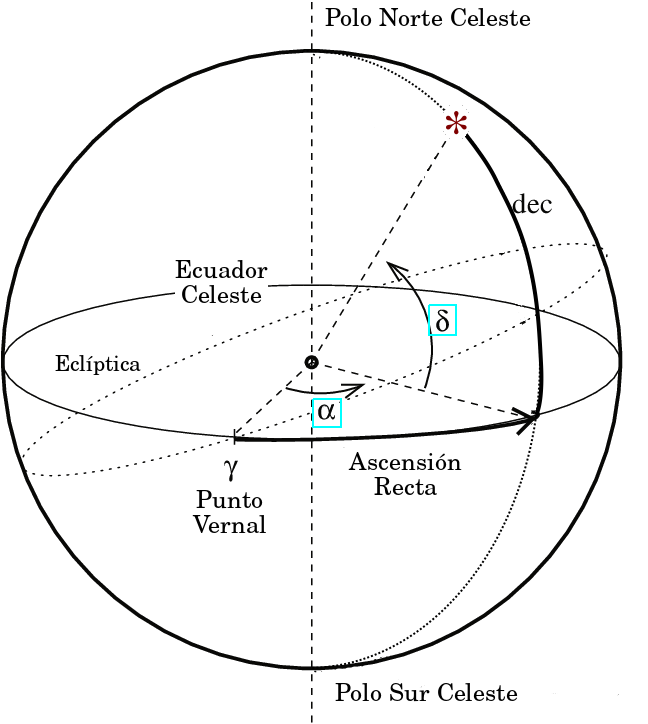
\includegraphics[width=0.6\textwidth]{EC.png}
        \end{center}
        \caption{}
        \label{fig:}
    \end{small}
\end{figure}


Las coordenadas ecuatoriales de un objeto cambian lentamente año tras año debido a la precesión del eje de rotación de la Tierra (con un período de $\sim$25770 años) con respecto a un eje perpendicular al plano de la eclíptica. Debido a que las coordenadas ecuatoriales están fijas al ecuador terrestre y relativas al equinoccio vernal, el sistema de coordenadas se mueve conforme la Tierra precede. La coordenadas de un objeto celeste cambiarán lentamente ( $\sim 1'$ por año) y es necesario entonces asignar una época para tales coordenadas.

\section{Coordenadas Locales} \label{apendice:local}

El sistema de coordenadas locales o también llamado coordenadas horizontales, localiza los objetos de acuerdo a un sistema centrado en la posición del observador. El ecuador en este sistema está definido por la intersección del plano tangente a la superficie de la Tierra en la ubicación del observador y la esfera celeste. 

La localización de un objeto está dada por dos ángulos: La altitud $a$ medida desde el plano ecuatorial en dirección al cenit del observador (el cenit corresponde al punto sobre la esfera celeste directamente arriba del observador y corresponde a una altitud de 90$^o$ ). Suele expresarse en lugar de la altitud el ángulo cenital $\theta$ que es el ángulo
complementario a la altitud; $\theta = 90^o - a$ . El segundo ángulo es el azimutal $\phi$ medido sobre el plano ecuatorial tomando como referencia algún punto, por ejemplo, el observatorio Pierre Auger define el cero hacia el Este y crece en dirección Norte (Anti-horario). La altitud mide ángulos entre -90$^o$ y 90$^o$ aunque la parte de altitud negativa no es visible por el observador. El azimut recorre desde 0$^o$ hasta 360$^o$. Se debe tener en cuenta además que este sistema al estar fijo con el observador se mueve con la rotación de la Tierra.


\begin{figure}[H]
    \begin{small}
        \begin{center}
            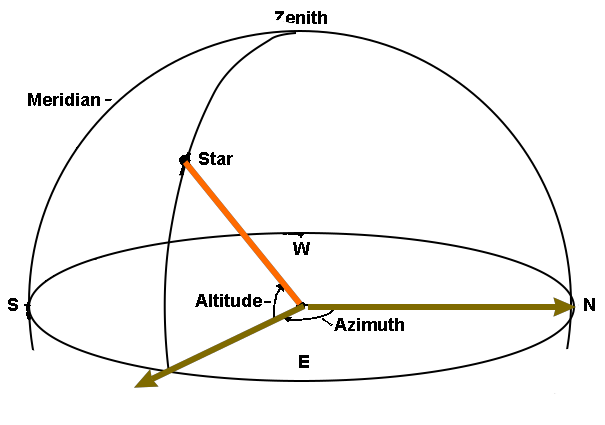
\includegraphics[width=0.75\textwidth]{LC.png}
        \end{center}
        \caption{}
        \label{fig:}
    \end{small}
\end{figure}


\subsection{Relación entre las coordenadas locales y ecuatoriales} \label{cambio_coord}
